\section{Introduction:}

The transistor is a three-layer semiconductor device consisting of either two n- and one p-type layers of material or two p- and one n-type layers of material. The former is called an {\bfseries\itshape npn transistor}, while the latter is called a {\bfseries\itshape pnp transistor}. Both are shown in Figure 1.0 with the proper dc biasing.

\begin{figure}[H]
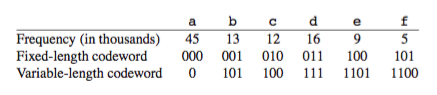
\includegraphics[scale=.5]{1.png}
\centering \linebreak \linebreak Figure 1.0: Transistor types. ( a ) pnp and ( b ) npn.
\end{figure}

\subsection{Transistor Operation:}

\begin{multicols}{2}
The basic operation of the transistor will now be described using the {\bfseries\itshape pnp transistor} of Figure 1.0a. The operation of the {\bfseries\itshape npn transistor} is exactly the same if the roles played by the electron and hole are interchanged. In Figure 1.1.0 the {\bfseries\itshape pnp transistor} has been redrawn without the base-to-collector bias. Note the similarities between this situation and that of the forward-biased diode in Practice 1. The depletion region has been reduced in width due to the applied bias, resulting in a heavy flow of majority carriers from the p- to the n-type material.

\begin{figure}[H]
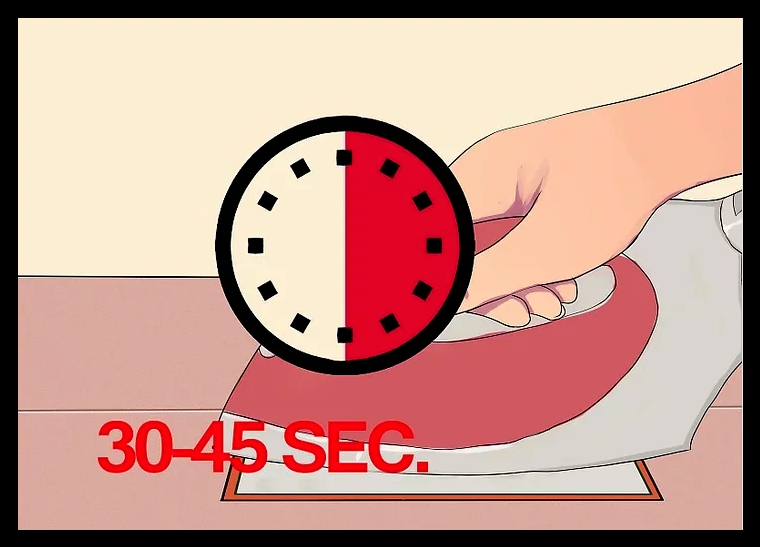
\includegraphics[scale=.5]{2.png}
\centering \linebreak \linebreak Figure 1.1.0: Forward-biased junction of a pnp transistor.
\end{figure}
\end{multicols}

\begin{multicols}{2}
Let us now remove the base-to-emitter bias of the {\bfseries\itshape pnp transistor} of Figure 1.0a as shown in Figure 1.1.1. Consider the similarities between this situation and that of the reverse-biased diode of Practice 1. Recall that the flow of majority carriers is zero, resulting in only a minority-carrier flow, as indicated in Figure 1.1.1. In summary, there- fore: \hfill \break

{\large\bfseries\itshape\color{carmine}{One p-n junction of a transistor is reverse biased, while the other is forward biased.}}

\begin{figure}[H]
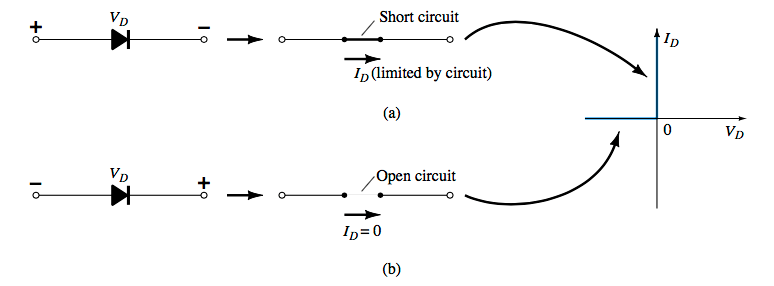
\includegraphics[scale=.5]{3.png}
\centering \linebreak \linebreak Figure 1.1.1: Reverse-biased junction of a pnp transistor.
\end{figure}
\end{multicols}

In Figure 1.1.2 both biasing potentials have been applied to a pnp transistor, with the resulting majority- and minority-carrier flow indicated. Note in Figure 1.1.2 the widths of the depletion regions, indicating clearly which junction is forward-biased and which is reverse-biased. As indicated in Figure 1.1.2, a large number of majority carriers will diffuse across the forward-biased p-n junction into the n-type material. The question then is whether these carriers will contribute directly to the base current $I_{b}$ or pass directly into the p-type material. Since the sandwiched n-type material is very thin and has a low conductivity, a very small number of these carriers will take this path of high resistance to the base terminal. The magnitude of the base current is typically on the order of microamperes as compared to milliamperes for the emitter and collector currents. The larger number of these majority carriers will diffuse across the reverse-biased junction into the p-type material connected to the collector terminal as indicated in Figure 1.1.2. The reason for the relative ease with which the majority carriers can cross the reverse-biased junction is easily understood if we consider that for the reverse-biased diode the injected majority carriers will appear as minority carriers in the n-type material. In other words, there has been an injection of minority carriers into the n-type base region material. Combining this with the fact that all the minority carriers in the depletion region will cross the reverse-biased junction of a diode accounts for the flow indicated in Figure 1.1.2.

\begin{figure}[H]
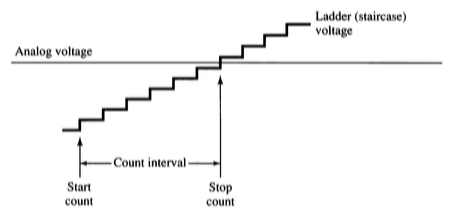
\includegraphics[scale=.6]{4.png}
\centering \linebreak \linebreak Figure 1.1.2: Majority and minority carrier flow of a pnp transistor.
\end{figure}

Applying Kirchhoff’s current law to the transistor of Figure 1.1.2 as if it were a single node, we obtain:

\begin{ceqn}
\begin{align}
I_{E} = I_{B} + I_{C}
\end{align}
\end{ceqn}

... and find that the emitter current is the sum of the collector and base currents. The collector current, however, is comprised of two components the majority and minority carriers as indicated in Figure 1.1.2. The minority-current component is called the leakage current and is given the symbol $I_{CO}$ ($I_{C}$ current with emitter terminal Open). The collector current, therefore, is determined in total by Equation ( 2 ):

\begin{ceqn}
\begin{align}
I_{C} = I_{C_{majority}} + I_{CO_{minority}}
\end{align}
\end{ceqn}

\subsection{Alpha $\alpha$:}

In the dc mode the levels of $I_{C}$ and $I_{E}$ due to the majority carriers are related by a quantity called {	\bfseries\itshape alpha} and defined by the following equation:

\begin{ceqn}
\begin{align}
\alpha_{dc} =\frac{I_{C}}{T_{E}}
\end{align}
\end{ceqn}

Where$I_{C}$ and $I_{E}$ are the levels of current at the point of operation. Even though the characteristics of the ideal transistor suggest that $\alpha$ = 1, for practical devices the level of alpha typically extends from 0.90 to 0.998, with most approaching the high end of the range. Since alpha is defined solely for the majority carriers, equation 2, becomes:

\begin{ceqn}
\begin{align}
I_{C} = \alpha I_{E} + I_{CBO}
\end{align}
\end{ceqn}

\pagebreak

\subsection{Common-Emitter Configuration:}

The most frequently encountered transistor configuration appears in Figure 1.3.0 for the pnp and npn transistors. It is called the common-emitter configuration since the emitter is common or reference to both the input and output terminals (in this case common to both the base and collector terminals). Two sets of characteristics are again necessary to describe fully the behavior of the common-emitter configuration: one for the input or base-emitter circuit and one for the output or collector-emitter circuit. Both are shown in Figure 1.3.1.

\begin{figure}[H]
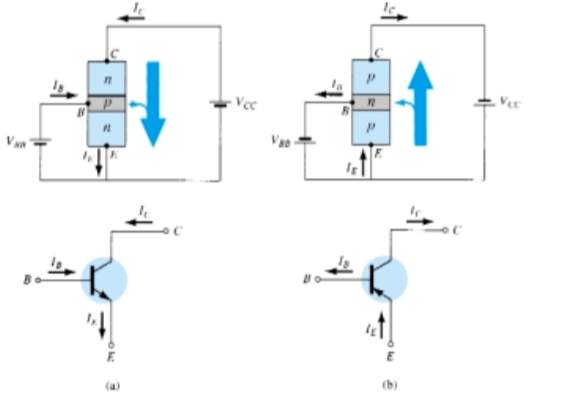
\includegraphics[scale=.6]{5.png}
\centering \linebreak \linebreak Figure 1.3.0: Notation and symbols used with the common-emitter configuration: (a) npn transistor; (b) pnp transistor.
\end{figure}

The emitter, collector, and base currents are shown in their actual conventional current direction. Even though the transistor configuration has changed, the current relations developed earlier for the common-base configuration are still applicable. That is equation 1 and 4. For the common-emitter configuration the output characteristics are a plot of the output current ($I_{C}$) versus output voltage ($V_{CE}$) for a range of values of input current ($I_{B}$). The input characteristics are a plot of the input current ($I_{B}$) versus the input voltage ($V_{BE}$) for a range of values of output voltage ($V_{CE}$).

\begin{figure}[H]
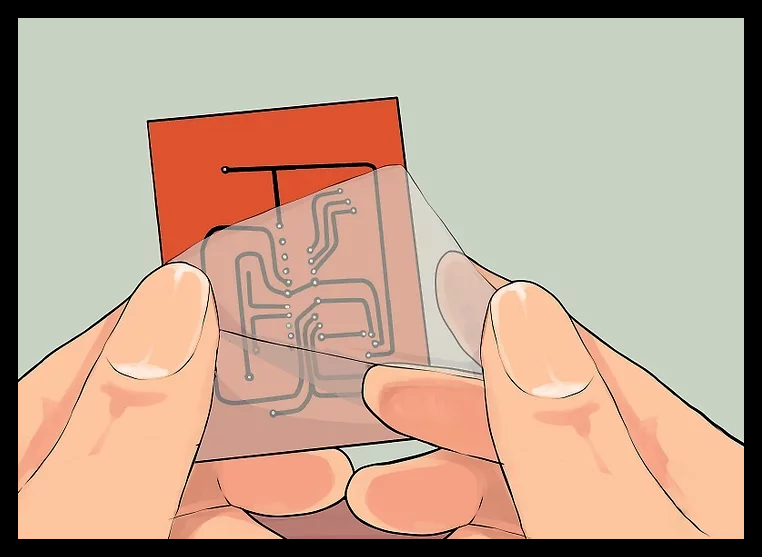
\includegraphics[scale=.55]{6.png}
\centering \linebreak \linebreak Figure 1.3.1: Characteristics of a silicon transistor in the common-emitter configuration: (a) collector characteristics; (b) base characteristics.
\end{figure}

\pagebreak

Note that on the characteristics of Figure 1.3.1 the magnitude of $I_{B}$ is in microamperes, compared to milliamperes of $I_{C}$. Consider also that the curves of $I_{B}$ are not as horizontal as those obtained for $I_{E}$ in the common-base configuration, indicating that the collector-to-emitter voltage will influence the magnitude of the collector current. \hfill \break 

{\large\bfseries\itshape\color{carmine}{In the active region of a common-emitter amplifier the collector-base junction is reverse-biased, while the base-emitter junction is forward-biased.}} \hfill \break

You will recall that these were the same conditions that existed in the active re- gion of the common-base configuration. The active region of the common-emitter configuration can be employed for voltage, current, or power amplification. The cutoff region for the common-emitter configuration is not as well defined as for the common-base configuration. Note on the collector characteristics of Figure 1.3.1 that $I_{C}$ is not equal to zero when $I_{B}$ is zero. For the common-base configuration, when the input current $I_{E}$ was equal to zero, the collector current was equal only to the reverse saturation current $I_{CO}$, so that the curve $I_{E}$ = 0 and the voltage axis were, for all practical purposes, one. The reason for this difference in collector characteristics can be derived through the proper manipulation of 1 and 4:

\begin{ceqn}
\begin{align}
I_{C} = \frac{\alpha I_{B}}{1 - \alpha} + \frac{I_{CBO}}{1 - \alpha}
\end{align}
\end{ceqn}

\subsection{Beta $\beta$:}

In the dc mode the levels of $I_{C}$ and $I_{B}$ are related by a quantity called beta and defined by the following equation:

\begin{ceqn}
\begin{align}
\beta_{dc} = \frac{I_{C}}{I_{B}}
\end{align}
\end{ceqn}

Where $I_{C}$ and $I_{B}$ are determined at a particular operating point on the characteristics. For practical devices the level of $\beta$ typically ranges from about 50 to over 400, with most in the midrange. As for $\alpha$, $\beta$ certainly reveals the relative magnitude of one cur- rent to the other. For a device with a $\beta$ of 200, the collector current is 200 times the magnitude of the base current. \hfill \break

A relationship can be developed between $\alpha$ and $\beta$ using the basic relationships introduced thus far. Using $\beta$ = $\frac{I_{C}}{I_{B}}$ we have $I_{B} = \frac{I_{C}}{\beta}$ and from $\alpha = \frac{I_{C}}{I_{E}}$ we have $I_{E} = \frac{I_{C}}{\alpha}$, such that:

\begin{ceqn}
\begin{align}
\alpha = \frac{\beta}{\beta + 1}
\end{align}
\end{ceqn}

\begin{ceqn}
\begin{align}
\beta = \frac{\alpha}{1 - \alpha}
\end{align}
\end{ceqn}

In addition, recall that: $I_{CEO} = \frac{I_{CBO}}{1 - \alpha}$, but using the equivalence: $\frac{1}{1 - \alpha} = \beta + 1$, we can say:

\begin{ceqn}
\begin{align}
I_{CEO} \cong \beta I_{CBO}
\end{align}
\end{ceqn}

As indicated on Figure 1.3.1. Beta is a particularly important parameter because it provides a direct link between current levels of the input and output circuits for a common-emitter configuration. From $I_{C} = \beta I_{B}$ and equation 1, we deduce:

\begin{ceqn}
\begin{align}
I_{E} = ( \beta + 1 ) I_{B}
\end{align}
\end{ceqn}

\pagebreak
